\documentclass{article}
\usepackage[utf8]{inputenc}
\usepackage{amssymb, amsmath, amsthm}
\usepackage{thmtools, mathtools, mathrsfs}
\usepackage{amsfonts}
\usepackage{stmaryrd}
\usepackage[sort&compress,numbers]{natbib}
\usepackage{subcaption}
\usepackage{graphicx}
\usepackage{caption}
\usepackage{float}
\usepackage{bm}

\newcommand{\defvec}[1]{\expandafter\newcommand\csname v#1\endcsname{{\mathbf{#1}}}}
\newcommand{\dm}[1]{\ensuremath{\mathrm{d}{#1}}} % dx dy dz dmu
\newcommand{\RN}[2]{\frac{\dm{#1}}{\dm{#2}}} % (Radon-Nikodym) derivative
\newcommand{\PD}[2]{\frac{\partial #1}{\partial #2}} % partial derivative
\newcommand{\mb}[1]{\mathbb{#1}}
\newcommand{\mc}[1]{\mathcal{#1}}
\DeclareMathOperator{\Inv}{Inv}
\DeclareMathOperator{\innt}{int}
\DeclareMathOperator{\relu}{ReLU}


\usepackage{tikz}
\usetikzlibrary{positioning,matrix,arrows,decorations.pathmorphing}
\usepackage{tikz-cd} 
% \usetikzlibrary{graphs,graphdrawing,arrows.meta}
% \usegdlibrary{circular}
\definecolor {processblue}{cmyk}{0.8,0,0,0}

\newcommand{\probP}{\text{I\kern-0.15em P}}

\newtheorem{theorem}{Theorem}
\newtheorem{prop}{Proposition}
\theoremstyle{definition}
\newtheorem{definition}{Definition}
\theoremstyle{remark}
\newtheorem{remark}{Remark}


\title{All line attractors are unstable, but some are more unstable than others}
% \title{All structurally unstable systems are unstable but some are more unstable than others}
% \title{Stability properties of sensory integration RNNs}
% Not all structurally unstable systems are created equal(ly unstable)
% \author{\'Abel S\'agodi}
\date{\today}



\begin{document}
\maketitle

\section*{Abstract}

Attractor networks play an essential role in computational neuroscience as a model for (perceptual) decision-making, memory and neural computation more generally.
It is well known that some of these networks, for example continuous attractor networks which can represent continuous variables, are structurally unstable.
This is a problem in biological neural networks because they are constantly undergoing perturbations caused by noise. %D-type.
We apply an existing result from dynamical systems theory to show that bounded attractors are stable in the following sense.
All perturbations of bounded attractors result in systems where the attractor (and its topology) is maintained. This has as consequence that if there is a restorative learning signal there are no exploding gradients for any time length (for backpropagation through time).
We contrast this to unbounded attractors that devolve into divergent systems under some perturbations which can lead to exploding gradients.
We work out a simple example and show that all perturbations preserve the attractor
and demonstrate the principle numerically in some systems relevant to neuroscience, namely the finite, ring and plane bump attractors.



%Even though ReLU RNNs can express a line attractor solution, not all solutions are robust to the learning process. There exists two types of solutions for perfect (with lossless, non-fading memory) integration in ReLU activated single layer RNN networks. We show that one of these types of solutions is more robust in the sense of more stable gradients. Although both networks go through bifurcations around the optimal parameters (which would result in exploding gradients), only one of the networks has solely bounded solutions for all parameter values in the neighborhood of this optimal set of parameters. Furthermore, we investigate the trade-off between the bounded integration potential of the bounded line attractor and the divergent instability of the perfect line attractor. 

%Finally, we relate this result to tolerance stability.





% Topics:
% Exploding gradients
% because of bifurcation 
% % https://citeseerx.ist.psu.edu/document?repid=rep1&type=pdf&doi=b57927b713a6f9b73c7941f99144165396483478
% \citep{doya1993}
% https://ieeexplore.ieee.org/document/230622




% Continuous attractors (necessary for ReLU perfect integration in a finite network)
% -Line
% -Surface

% Fine tuning 

% ReLU


% Solutions
% Initialization
% - Identity
%     -- Fine tuning problem
%         ---Not the same for all fine tuned networks!




% links to relevance:
% mutual inhibition with external excitation is more stable than excitatory networks 


% While in principle the recurrent network is a simple and powerful model, in practice, it is unfortunately hard to train properly due  to vanishing and exploding gradients. 
% %
% One of the main category of methods that have been proposed to improve the speed of training and the quality of it's result is to choose a suitable initialization for the parameters. One such proposal is to have the identity matrix as the initial parameters for the recurrent weights, which is especially suitable to help with learning long term dependencies \citep{Le2015}.
%

%
% Here, we study the gradient characteristics in the neighbourhood of the parameter space around the different solutions.
%
% There exists two types of solutions for perfect\footnote{Lossless/non-fading.} integration in ReLU activated single layer RNN networks.
% %
% We show that one of these types of solutions is more robust in the sense of more stable gradients.
% %
% Although both networks go through bifurcations around the optimal parameters (which would result in exploding gradients \citep{doya1993bif}), only one of the networks has solely bounded solutions for all parameter values in the neighbourhood of this optimal set of parameters.
% The more stable set of parameters corresponds to mutual inhibition with external excitation \citep{myre1993, machens2005}. 
% Furthermore, we investigate the trade-off between the bounded integration potential of the bounded line attractor and the divergent instability of the perfect line attractor.



% Bifurcations cause exploding gradients \citep{pascanuDifficultyTrainingRecurrent2013}





% Tolerance stability
% \cite{zeeman1962}

% \citep{ikegamiExistenceToleranceStable1983}


\newpage 
\section{Introduction}





\subsection{Gradients}

Back-Propagation Through Time (BPTT, e.g., [22, 27, 26])  tend to either (1) blow up or (2) vanish:
 the temporal evolution of the backpropagated error exponentially depends on the size of the weights [11, 6]. 

Case (1) may lead to oscillating weights

\subsection{RNNs}

\citep{vogtLyapunovExponentsRNNs2022}

\citep{kolenGradientFlowRecurrent2009}




\subsubsection{Exploding}

Continuous attractor dynamics, a previously known solutions to the EVGP, often suffer from the \emph{fine tuning problem}---small change in the parameters can drastically reduce the effectiveness.

An exact line attractor can be easily designed and implemented, for example, LDS with null eigenvalues and LSTM with no forgetting.

 the realization of line attractors are fragile to parameter changes ~\citep{seung1998,goldman2003}.

Similar phenomenon has also been observed in GRU networks which simplifies the LSTM by removing the linear cell structure~\citep{jordan2021}.
A notable exception is the ring attractor which can be implemented using bump attractor network architecture, also seen in the biological neural system.
However, stable oscillations are much more robust to parameter perturbations.




\subsubsection{Activation functions}
\citep{clevertFastAccurateDeep2016b}


\subsection{Bifurcations}

In dynamical systems, when infinitely small change in the parameters cause a qualitative change in the dynamics due to changes in the topology of the dynamics, it is said that the system undergoes a bifurcation.

The asymptotic behavior of a recurrent neural network changes qualitatively at certain points in the parameter space, which are known as \emph{bifurcation points}.



At bifurcation points, the output of a network can change discontinuously with the continuous change of parameters and therefore convergence of gradient descent algorithms is not guaranteed in such cases.


Furthermore, learning equations used for error gradient estimation can be unstable


If we randomly pick one point in the parameter space, it is very unlikely that it is a bifurcation point. However, it we change the parameters continuously by learning, there is a non-negligible chance that we encounter codimension-one bifurcations.

The parameter space of a recurrent network is divided into many regions with different qualitative structure of the
state space, for example, the regions in which the state space has only one attractor point, one limit cycle, two attractor points, one attractor point and one limit cycle, and so on. Those qualitatively different regions are bordered by bifurcation points. Therefore, some types of bifurcations are inevitable steps in constructing a network with an interesting dynamical behavior. However, when the network goes through a bifurcation, either purposefully or by a mishap, gradient descent algorithms can have problems as shown below.


If a gradient descent algorithm with a fixed learning rate is used, a very large error gradient causes a long jump in the parameter space. It can even lead to a numerical overfow.
 Even if those are not the case, gradient descent does not work effciently when the size of gradient varies so much in different directions.

\subsubsection{Codimension-one}

In general, bifurcations occur when the vector eld F satises some constraints.

 The above cases can be seen on a k-1 dimensional surface in k dimensional parameter space and therefore called codimension-one bifurcations

%\subsubsection{Types of system}
%Piecewise-smooth dynamical systems \citep{dibernardoPiecewisesmoothDynamicalSystems2008}

\subsection{Bifurcations of Recurrent Neural Networks}
\citep{doyaBifurcationsRecurrentNeural}



%\newpage 
\section{Stability concepts}



\subsection{Structural stability}
In addition to the S-type noise, biological neural systems have constantly fluctuating synaptic weights~\cite{Shimizu2021}.
In other words, there is noise in the recurrent network dynamics, which we call the \emph{D-type noise}.

An important consequence of the presence of D-type noise is that the neural computation implemented by recurrent dynamics is constantly fluctuating.
Therefore, the desirable properties of the dynamical system that require precise weight combinations are not stably achievable due to their unreliability.

The topological structures that are robust under D-type noise are called \emph{structurally stable} -- for example, a stable fixed point is structurally stable~\cite{Kuznetsov1995}.


Unfortunately, continuous attractors are not structurally stable -- small changes in the dynamical system can destroy continuous attractors, and as a consequence, the corresponding Lyapunov exponent(s) move away from zero.
For example, in machine learning, vanilla RNNs are sometimes initialized at the continuous attractor regime with all zeros such that 
%$\RN{\vx}{t} = \mathbf{0}$,
 which avoids the asymptotic EVGP initially, but very quickly loses the continuous attractor after one gradient step.
This is a well known problem in neuroscience, often referred to as the ``fine tuning problem'' of the continuous attractor~\cite{Seung1996,Renart2003,Noorman2022}.
There have been remedies to lesson the degradation, often focusing on keeping the short-term behavior close to the continuous attractor case~\cite{Lim2012,Lim2013,Boerlin2013,Koulakov2002}.

% \subsection{Tolerance stability}


\subsection{Initialization}

%Preprogramming of the state space
When we have an a priori knowledge about the required qualitative structure of the state space, for example, the number of attractors, it is possible to preprogram it by the initial connection weights. For example, if we want to train a network to have multiple limit cycle attractors, it is helpful to set the initial connection weights to have multiple attractor points. % using autocorrelation matrix [6]. 

%In such a case, problems with saddle-node bifurcations are avoided and changing fixed points into limit cycles is not diffcult if teacher forcing is used, as described later.

%%Actually in many cases, recurrent networks are trained as an adaptive nonlinear filters[1, 17, 15]. In these cases, the main issue of learning is to t the transient response of the network to the desired curves and the network should have a single attractor point. This can be realized without any bifurcations from weak random initial connections. Convergence of gradient descent learning is theoretically guaranteed in this case [16].






\section{Perfect integrator}
The MSE on the whole trial is 
\[
\frac{1}{T}\int_0^T \left( h(t) - \int_0^t x(\tau)d\tau\right)^2 dt,
\]
with \[x(t) = \sum_{i=1}^{\# R}\delta(t-R(i))-\sum_{i=1}^{\# L}\delta(t-L(i))\] the input at time $t$ where $\#R$ and $\#L$ are the number of right and left clicks up to time $t$, respectively and $R(i)$ and $L(i)$ are the timings of the $ith$ right and left clicks respectively. 

Assuming the parameters of the perfect one-dimensional integrator (with $\theta=1$)
% \[
% h(t+\Delta t) = \theta h(t) + x(t)
% \]
% \[
% \frac{h(t+\Delta t)-  h(t)}{\Delta t} = (\theta - 1)h(t) + x(t),
% \]
% \begin{equation}\label{eq:dhdt}
% \frac{dh}{dt} = (\theta - 1)h(t) + x(t)    
% \end{equation}
\begin{equation}\label{eq:dhdt}
\frac{dh}{dt} = -\lambda h(t) + x(t)    
\end{equation}
the MSE on the whole trial is zero.

The solution to \eqref{eq:dhdt} is
\begin{equation}
    h(t) = \sum_{i=1}^{\# R}e^{\lambda(t-R(i))}-\sum_{i=1}^{\# L}e^{\lambda(t-L(i))},
\end{equation}
with $\lambda=-(\theta-1)$.

The integral of the inputs is
\[
\int_0^t x(\tau)d\tau = h(t) = \sum_{i=1}^{\# R}1-\sum_{i=1}^{\# L}1
\]

So then the MSE is
\[
\frac{1}{T}\int_0^T \left(\sum_{i=1}^{\# R}(e^{\lambda(t-R(i))}-1)-\sum_{i=1}^{\# L}(e^{\lambda(t-L(i))}-1)\right)^2 dt
\]


\[
\frac{1}{T}\int_0^T \left(\sum_{i=1}^{\# R + \#L}(-1)^{p(i)}(e^{\lambda(t-R(i))}-1)\right)^2 dt
\]

\[
\frac{1}{T}\int_0^T \left(\sum_{i=1}^{\# R + \#L}(-1)^{p(i)}(e^{\lambda(t-R(i))})-\sum_{i=1}^{\# R + \#L}(-1)^{p(i)}\right)^2 dt
\]

\subsection{Single click trial}
On a trial with a single click with the click time $t=C(1)$ with $C\in\{L,R\}$ we have
\begin{align*}
&\frac{1}{T-C(1)}\int_{C(1)}^{T} \left(e^{\lambda(t-C(1))}-1\right)^2 dt\\
&= \frac{3 - 4 e^{\lambda (T-C(1))} + e^{2 \lambda (T-C(1))} + 2 \lambda (T-C(1))}{2 \lambda(T-C(1))}
\end{align*}
% In the case that $\lambda>0$ the error grows exponentially.
In that case 
\begin{align*}
&\frac{\partial}{\partial \lambda}\frac{3 - 4 e^{\lambda (T-C(1))} + e^{2 \lambda (T-C(1))} + 2 \lambda (T-C(1))}{2 \lambda(T-C(1))}\\
&= \frac{ 4 (T-C(1)) e^{\lambda (T-C(1))} + 2(T-C(1))e^{2 \lambda (T-C(1))}}{2 \lambda(T-C(1))} -\frac{3+ 4 e^{\lambda (T-C(1))} + e^{2 \lambda (T-C(1))} }{ \lambda^2}\\
\end{align*}
Which causes exploding gradients.


\subsection{Two  click trial}
The integral from first click at $t=C(1)$ to the second click at $t=C(2)$ with $C\in\{L,R\}$ is
\begin{align*}
&\frac{1}{C(2)-C(1)}\int_{C(1)}^{C(2)} \left(e^{\lambda(t-C(1))}-1\right)^2 dt\\
&=\frac{1}{C(2)-C(1)}\int_{0}^{C(2)-C(1)} \left(e^{\lambda t}-1\right)^2 dt\\
&= \frac{3 - 4 e^{\lambda (C(2)-C(1))} + e^{2 \lambda (C(2)-C(1))} + 2 \lambda (C(2)-C(1))}{2 \lambda(C(2)-C(1))}
\end{align*}

If the direction of the second click is the same as the first, the integral from the second up to the third click is
\begin{align*}
&\frac{1}{C(3)-C(2)}\int_{0}^{C(3)-C(2)} \left(e^{\lambda(t-C(1)+C(2))}+e^{\lambda t}-2\right)^2 dt\\
%=& well this is already getting pretty ugly
\end{align*}


If the direction of the second click is the opposite as the first, the integral from the second up to the third click is
\begin{align*}
&\frac{1}{C(3)-C(2)}\int_{0}^{C(3)-C(2)} \left(e^{\lambda(t-C(1)+C(2))}-e^{\lambda t}\right)^2 dt\\
&=\frac{1}{C(3)-C(2)}\left[\frac{e^{-2 \lambda} (-1 + e^{2 S \lambda})}{2 \lambda} - \frac{2 e^{- \lambda} (-1 + e^{S(1 + \lambda)})}{1 + \lambda}+ e^S \sinh(S)\right]
\end{align*}
with $S=C(3)-C(2)$


A lower bound can be found by evaluating the case that at each consecutive click is opposite and we take the limit $C(i+1)-C(i)\rightarrow\infty$, in which case MSE=0.

\section{Noisy gradient descent}
We now look at a perturbation of the parameter of the linear integrator around $\theta=1$ or equivalently $\lambda=0$.

\begin{align*}
\frac{\partial}{\partial \lambda}&\frac{1}{T}\int_0^T \left(\sum_{i=1}^{\# R}(e^{\lambda(t-R(i))}-1)-\sum_{i=1}^{\# L}(e^{\lambda(t-L(i))}-1)\right)^2 dt\\
&= \frac{2}{T}\int_0^T \left[\sum_{i=1}^{\# R}(t-R(i))e^{\lambda(t-R(i))}-\sum_{i=1}^{\# L}(t-L(i))e^{\lambda(t-L(i))}\right] \left[\sum_{i=1}^{\# R}(e^{\lambda(t-R(i))}-1)-\sum_{i=1}^{\# L}(e^{\lambda(t-L(i))}-1)\right] dt\\
\end{align*}

If $\lambda>0$, i.e. if $\theta>1$,
if the last time point $t=R(i)$ of the stimulus has a right click (and no left click)
we get a contribution of 
\begin{align*}
& \frac{2}{T}\int_{R(i)}^T (t-R(i))e^{\lambda(t-R(i))}(e^{\lambda(t-R(i))}-1) dt\\
&= \frac{2}{T}\int_0^{T-R(i)} te^{\lambda t}(e^{\lambda t}-1) dt\\
\end{align*}

%
%\section{Spectral normalization}
%% Lipschitz 
%\begin{definition}
%A function $f\colon R^{M} \rightarrow R^{N}$ is Lipschitz continuous if there is a constant L such that $\|f(x) - f(y)\|  \leq  L \|x - y\|$ for every $x, y$.
%\end{definition}
%
%The smallest such L is the Lipschitz constant of $f$ and is denoted $Lip(f)$.
%
%Lipschitz continuity also has the following property:
%
%Let $f = g \circ h$. If $g$ and $h$ are Lipschitz continuous, then $f$ is also Lipschitz continuous with $Lip(f) \leq Lip(g) Lip(h)$.
%
%
%%applied to NNs
%$f$ is a neural network, and we want it to be Lipschitz continuous with a small $Lip(f)$.
%
%Functions commonly used in neural networks such as ReLU, sigmoid, softmax, tanh, max-pooling, have Lipschitz constant = 1.
%
%For simplicity we omit the bias term, so $FC(x) = Wx$ for some weight matrix W. It can be shown that FC has Lipschitz constant $Lip(FC) = \sigma(W)$ the spectral norm of W, which is equivalent to the largest singular value of W. Hence in general, $Lip(FC)$ can be arbitrarily large.
%
%Spectral Normalization comes into play by normalizing the spectral norm of W:
%\[W \mapsfrom W / \sigma(W)\]
%The normalized matrix has spectral norm = 1, thus Lip(FC) is also 1.










\section{Another implementation of a perfect integrator}

\subsection{Parameters of the integrator part}
\subsubsection{Input}
Parameter that determines step size along line attractor $\delta<<1$.
The size determines the maximum number of clicks as the difference between the two channels. 

This pushes the input along the line "attractor" in two opposite directions, %what is the correct word for this type of invariant set?
see below.

\begin{equation}\label{eq:bla}
\dot x = \relu(Wx+b) -x
\end{equation}

Recurrent
\begin{equation}
W = 
\begin{pmatrix}
0  &  -1 \\
-1  &  0
\end{pmatrix}
\end{equation}
%for $\alpha>0$.

Bias:
\begin{equation}
b = 
\begin{pmatrix}
1 \\  1 
\end{pmatrix}
\end{equation}

Output


%Discrete 
\subsubsection{Workings}
Maximally invariant set:
\[ [0,1]^2\]

Every point outside of this set gets mapped as
\[
(x,y) \mapsto
\begin{cases}
(1-y,0) \text{ if } y<1 \text{ and } x>1\\
(0,1-x) \text{ if } y>1 \text{ and } x<1\\
(0,0) \text{ if } y>1 \text{ and } x>1
\end{cases}
\]

Line attractor (not an isolated invariant set and also not really an attractor)
\[ \{(a,1-a) | a\in[0,1]\}\]

Outside of the line attractor


\subsubsection{Parameters of the full network part}
%i.e. INCLUDING reset + output trigger



\subsubsection{Learning from this initialization}







\newpage

\section{Accumulator systems}
\subsection{Line attractor}
We apply the perturbation
\begin{equation}
W' = 
\begin{pmatrix}
0  &  1 \\
1  &  0
\end{pmatrix}
+ \epsilon
\end{equation}
with 
\begin{equation}
\epsilon = 
\begin{pmatrix}
\epsilon_{11}  &  \epsilon_{12} \\
\epsilon_{21}  &  \epsilon_{22}
\end{pmatrix}
\end{equation}


The eigenvalues are computed as
\begin{align*}
\det [W' -(1+\lambda)\mathbb{I}] &= (\epsilon_{11}-1-\lambda)(\epsilon_{22}-1-\lambda)-(\epsilon_{12}+1)(\epsilon_{21}+1)\\
&=\lambda^2 - (2+\epsilon_{11}+\epsilon_{22})\lambda -\epsilon_{11}-\epsilon_{22}+\epsilon_{11}\epsilon_{22} -\epsilon_{12} - \epsilon_{21} - \epsilon_{12}\epsilon_{21}
\end{align*}

Let 
$u=- (2+\epsilon_{11}+\epsilon_{22})$
and 
$v=-\epsilon_{11}-\epsilon_{22}+\epsilon_{11}\epsilon_{22} -\epsilon_{12} - \epsilon_{21} - \epsilon_{12}\epsilon_{21}$

\begin{figure}[H]
    \centering
    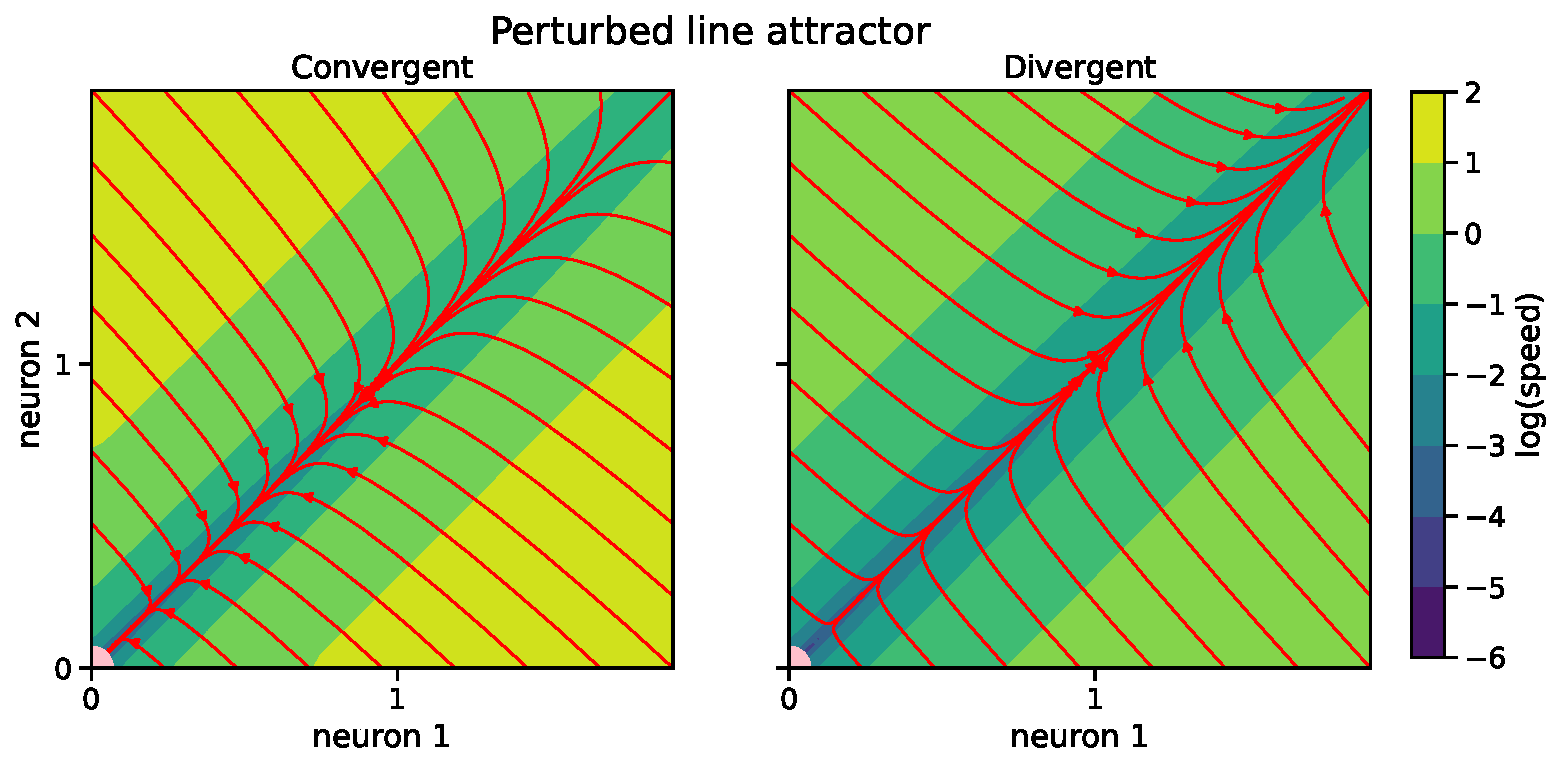
\includegraphics[width=0.99\textwidth]{figures/lineattractor_pert2.pdf}
    \caption{All types of perturbations for the bounded line attractor.}
    \label{fig:lineattractor_pert2}
\end{figure}

There are only two types of invariant set for the perturbations of the line attractor. Both have as invariant set a fixed point at the origin. What distinguishes them is that one type of perturbations lead to this fixed point being stable while the other one makes it unstable, see Figure \ref{fig:lineattractor_pert2}.

\subsection{Bounded line attractor}
\subsubsection{Definition}

\section{Lyapunov spectrum}
We investigate how perturbations to the bounded line affect the Lyapunov spectrum.
The Jacobian 
\begin{equation}
J = -
\begin{pmatrix}
1  &  1 \\
1  &  1
\end{pmatrix}
\end{equation}

We apply the perturbation
\begin{equation}
W' = 
\begin{pmatrix}
0  &  -1 \\
-1  &  0
\end{pmatrix}
+ \epsilon
\end{equation}
with 
\begin{equation}
\epsilon = 
\begin{pmatrix}
\epsilon_{11}  &  \epsilon_{12} \\
\epsilon_{21}  &  \epsilon_{22}
\end{pmatrix}
\end{equation}

The eigenvalues are computed as
\begin{align*}
\det [W' -(1+\lambda)\mathbb{I}] &= (\epsilon_{11}-1-\lambda)(\epsilon_{22}-1-\lambda)-(\epsilon_{12}-1)(\epsilon_{21}-1)\\
&=\lambda^2 - (2+\epsilon_{11}+\epsilon_{22})\lambda -\epsilon_{11}-\epsilon_{22}+\epsilon_{11}\epsilon_{22} +\epsilon_{12} + \epsilon_{21} - \epsilon_{12}\epsilon_{21}
\end{align*}

Let 
$u=- (2+\epsilon_{11}+\epsilon_{22})$
and 
$v=-\epsilon_{11}-\epsilon_{22}+\epsilon_{11}\epsilon_{22} + \epsilon_{12} + \epsilon_{21} - \epsilon_{12}\epsilon_{21}$

\begin{equation}
\lambda = \frac{-u \pm \sqrt{u^2-4v}}{2}
\end{equation}



Case 1: $\operatorname{Re}(\sqrt{u^2-4v})<u$, then 
$\lambda_{1,2}<0$


Case 2:  $\operatorname{Re}(\sqrt{u^2-4v})>u$, then 
$\lambda_{1}<0$ and $\lambda_{2}>0$


Case 3: $v=0$, then 
$\lambda=\tfrac{1}{2}(-u\pm u)$, i.e.,
$\lambda_1=0$ and  $\lambda_2=-u$

\begin{align}
\epsilon_{11} &= -\epsilon_{22}+\epsilon_{11}\epsilon_{22} + \epsilon_{12} + \epsilon_{21} - \epsilon_{12}\epsilon_{21}
\end{align}




\begin{figure}[H]
    \centering
    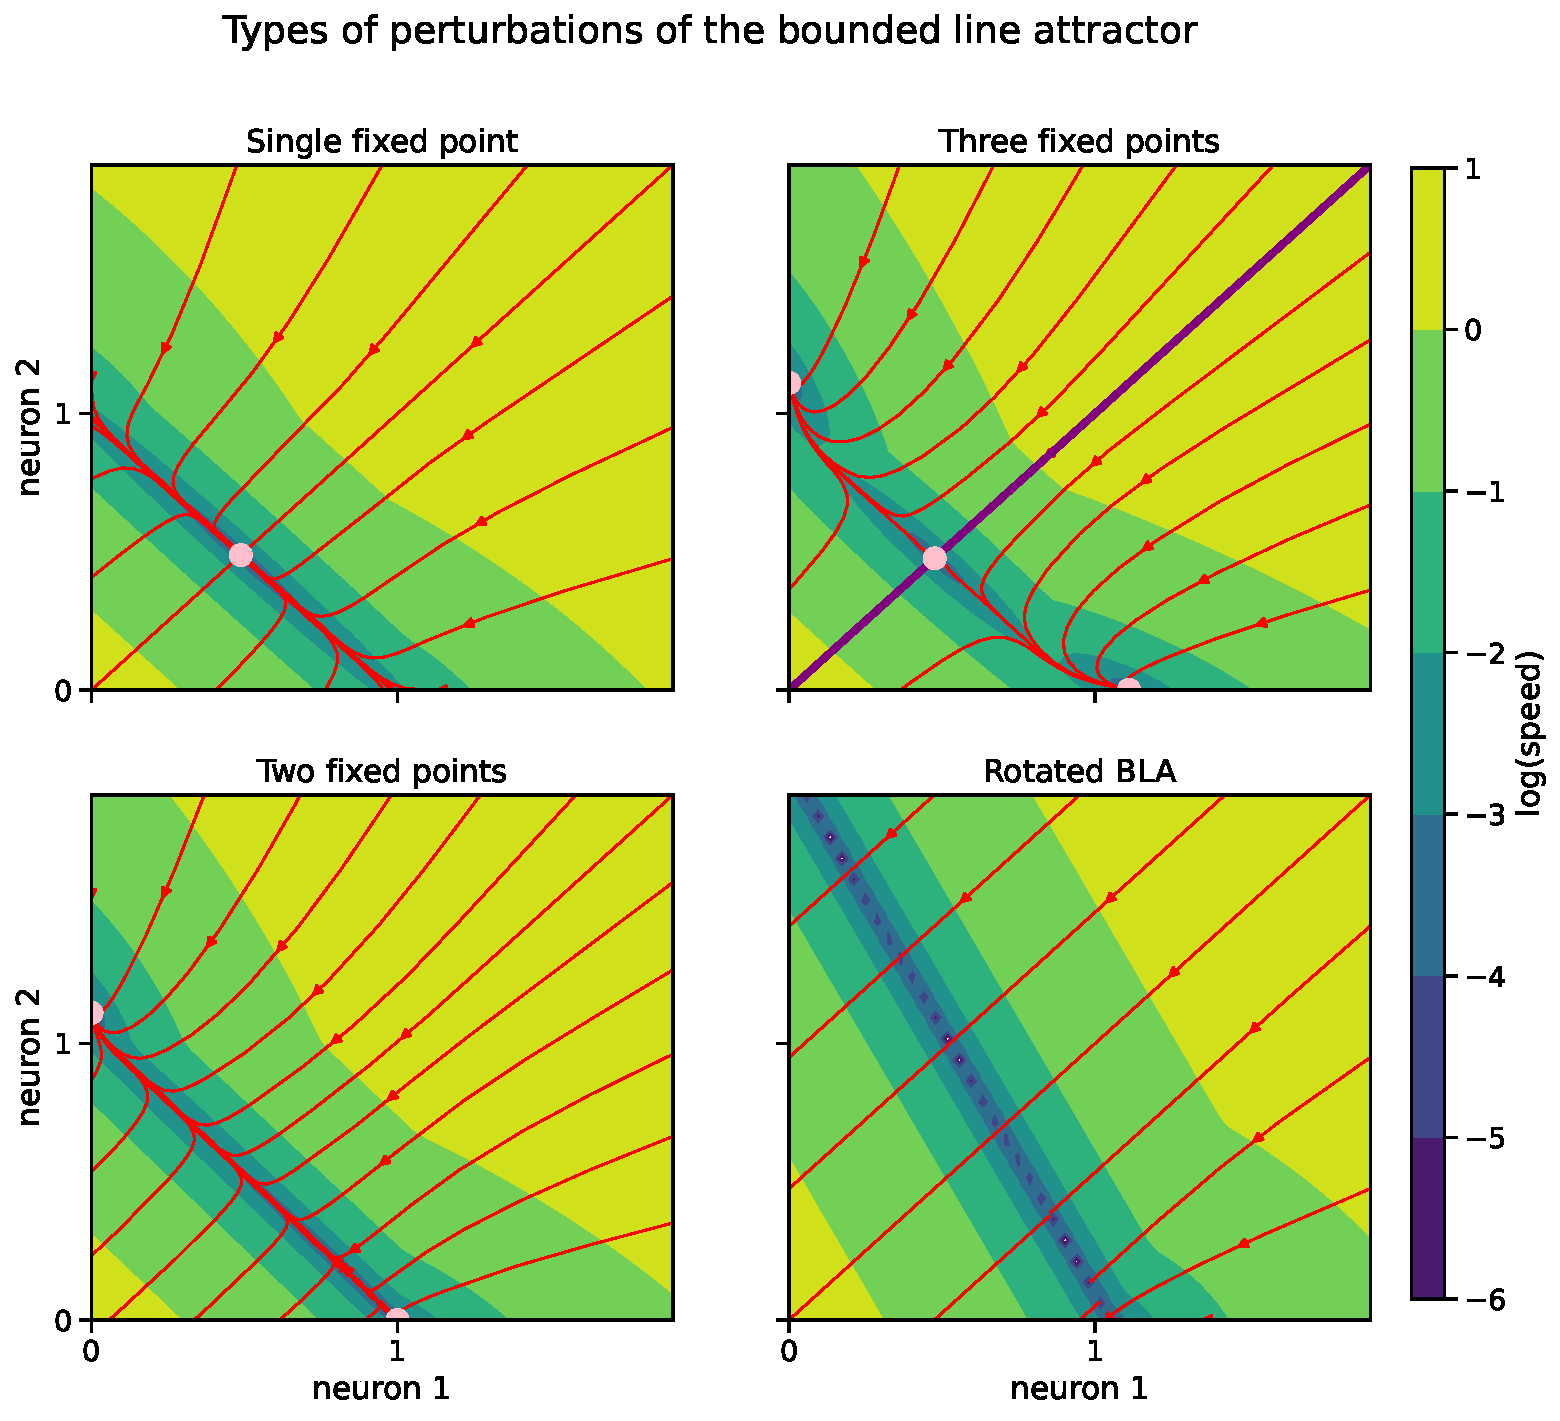
\includegraphics[width=0.99\textwidth]{figures/bounded_lineattractor_allpert.pdf}
    \caption{All types of perturbations for the line attractor.}
    \label{fig:bounded_lineattractor_allpert}
\end{figure}


We give some examples of the different types of perturbations to the bounded line attractor.
The first type is when the invariant set is composed of a single fixed point, for example for the perturbation:
\begin{equation}
\epsilon = \frac{1}{10}
\begin{pmatrix}
-2  &  1 \\
 1   &  -2
\end{pmatrix}
\end{equation}
See Figure \ref{fig:bounded_lineattractor_allpert}, left upper.



The second type is when the invariant set is composed of three fixed points:
\begin{equation}
\epsilon = \frac{1}{10}
\begin{pmatrix}
1  &  -2 \\
 -2  &  1
\end{pmatrix}
\end{equation}

The third type is when the invariant set is composed of two fixed points, both with partial support.
\begin{equation}
b' =  \frac{1}{10}
\begin{pmatrix}
1 & -1
\end{pmatrix}
\end{equation}

The fourth and final type is when the line attractor is maintained but rotated:
\begin{equation}
\epsilon =  \frac{1}{20}
\begin{pmatrix}
1 & 10\\
10 & 1
\end{pmatrix}
\end{equation}

\begin{theorem}
All perturbations of the bounded line attractor are of the types as listed above.
\end{theorem}



\begin{proof}
We enumerate all possibilities for the dynamics of a ReLU activation network with two units.
First of all, note that there can be no limit cycle or chaotic orbits.

Now, we look at the different possible systems with fixed points.
There can be at most three fixed points \citep[Corollary 5.3]{morrisonDiversityEmergentDynamics2022}.
There has to be at least one fixed point, because the bias is non-zero.

%1 fixed point
General form (example):
\begin{equation}
\epsilon = \frac{1}{10}
\begin{pmatrix}
-2  &  1 \\
 1   &  -2
\end{pmatrix}
\end{equation}

One fixed point with full support:

In this case we can assume $W$ to be full rank.

\begin{align*}
\dot x = 
\relu\left[
\begin{pmatrix}
\epsilon_{11}  &  \epsilon_{12} \\
\epsilon_{21}  &  \epsilon_{22}
\end{pmatrix}
\begin{pmatrix}
x_1\\x_2
\end{pmatrix}
+
\begin{pmatrix}
1\\1
\end{pmatrix}
\right]
-
\begin{pmatrix}
x_1\\x_2
\end{pmatrix}
&=0
\end{align*}


Note that $x>0$ iff $z_1\coloneqq \epsilon_{11}x_1 + (\epsilon_{12}-1)x_2-1>0$. Similarly for $x_2>0$.

So for a fixed point with full support, we have 
\begin{equation}
\begin{pmatrix}
x_1\\x_2
\end{pmatrix}
=A^{-1}
\begin{pmatrix}
-1\\-1
\end{pmatrix}
\end{equation}
with 
\[A\coloneqq\begin{pmatrix}
\epsilon_{11}-1  &  \epsilon_{12}-1 \\
\epsilon_{21}-1  &  \epsilon_{22}-1
\end{pmatrix}.\]


Note that it is not possible that $x_1=0=x_2$.

Now define
\[
B\coloneqq A^{-1} = \frac{1}{\det A}
\begin{pmatrix}
\epsilon_{22}-1  &  1-\epsilon_{12} \\
1-\epsilon_{21}  &  \epsilon_{11}-1
\end{pmatrix}
\]
with \[\det A = \epsilon_{11}\epsilon_{22}-\epsilon_{11}-\epsilon_{22}+\epsilon_{12}\epsilon_{21}-\epsilon_{12}-\epsilon_{21}.\]

Hence, we have that $x_1,x_2>0$ if $B_{11}+B_{12}>0$, $B_{21}+B_{22}>0$ and $\det A >0$ 
and $B_{11}+B_{12}<0$, $B_{21}+B_{22}<0$ and $\det A <0$.

If $\det A >0$, this is satisfied if $\epsilon_{22}>\epsilon_{12}$ and $\epsilon_{11}>\epsilon_{21}$,
while if $\det A >0$, this is satisfied if $\epsilon_{22}<\epsilon_{12}$ and $\epsilon_{11}<\epsilon_{21}$.
This gives condition 1. %necessary condition (#1)



Finally, we investigate the condition that specify that there are no fixed points with partial support.
%condition for no fixed points for which $x_i=0$ for i=1 or i=2 (necessary condiiton #2)


If $x_1=0$ then $(\epsilon_{22}-1)x_2+1=0$ and $z_1<0$. 
From the equality, we get that $x_{2}=\frac{1}{1-\epsilon_{22}}$.
From the inequality, we get  $(\epsilon_{12}-1)x_2+1\geq 0$, i.e. $\frac{1}{1-\epsilon_{12}}\geq x_2$.
Hence, 
\begin{equation*}
\frac{1}{1-\epsilon_{12}}\geq\frac{1}{1-\epsilon_{22}}
\end{equation*}
and thus
\begin{equation}\label{eq:condition2.1}
\epsilon_{22} \leq \epsilon_{12}.
\end{equation}

Similiarly, we have that 
\begin{equation}\label{eq:condition2.2}
\epsilon_{11} \leq \epsilon_{21}.
\end{equation}

Equation \ref{eq:condition2.1} and \ref{eq:condition2.2} together form condition 2.

%2 fixed points
If condition 1 is violated, there are two fixed points on the boundary of the admissible quadrant.
%what about the subconditions?

%3 fixed points
If condition 2 is violated, there are three fixed points.
%what about the subconditions?


We now look at the possibility of the line attractor being preserved. 
This is the case if $v=0$.
It is not possible to have a line attractor with a fixed point off it for as there cannot be disjoint fixed points that are linearly dependent \citep[Lemma 5.2]{morrisonDiversityEmergentDynamics2022}.
\end{proof}






\subsection{Structure of the parameter space}

We check what proportion of the bifurcation parameter space is constituted with bifurcations of the type that result in three fixed points.

The conditions are 
\begin{align*}
0 &< \epsilon_{11}\epsilon_{22}-\epsilon_{11}-\epsilon_{22}+\epsilon_{12}\epsilon_{21}-\epsilon_{12}-\epsilon_{21},\\
\epsilon_{22} &\leq \epsilon_{12},\\
\epsilon_{11} &\leq \epsilon_{21}.
\end{align*}


We show that if 
\begin{align*}
\epsilon_{22} &\leq \epsilon_{12},\\
\epsilon_{11} &\leq \epsilon_{21}.
\end{align*}
then always 
\begin{align*}
0 &< \epsilon_{11}\epsilon_{22}-\epsilon_{11}-\epsilon_{22}+\epsilon_{12}\epsilon_{21}-\epsilon_{12}-\epsilon_{21}.
\end{align*}










\newpage
\section{Bounded plane attractor}
%https://www.wolframalpha.com/input?i=inverse+%5B%5Ba-1%2Cb-1%2Cc-1%5D%2C%5Bd-1%2Ce-1%2Cf-1%5D%2C%5Bg-1%2Ch-1%2Ci-1%5D%5D/

\begin{equation}
W = 
\begin{pmatrix}
0  &  -1 & -1\\
-1  &  0 & -1\\
-1 &  -1 & 0	
\end{pmatrix}
\end{equation}
and
\begin{equation}
b = 
\begin{pmatrix}
1  \\
1 \\
1\\
\end{pmatrix}
\end{equation}

\begin{equation}
\epsilon = 
\begin{pmatrix}
\epsilon_{11}  &  \epsilon_{12} & \epsilon_{13}\\
\epsilon_{21}  &  \epsilon_{22} & \epsilon_{23}\\
\epsilon_{31}  &  \epsilon_{32} & \epsilon_{33}
\end{pmatrix}
\end{equation}

\subsection{Limit cycle}

\citep[Theorem 2.4]{morrison} 
$G$ be an oriented graph with no sinks
If $\epsilon<\tfrac{\delta}{1+\delta}$, then the network has bounded activity and no stable fixed points.

\subsubsection{With one fixed point}
\begin{equation}
\epsilon = 
\begin{pmatrix}
 0  &  -\delta_1 & \delta_2 \\
 \delta_2  &  0 & -\delta_1 \\
-\delta_1 & \delta_2 & 0 \\
\end{pmatrix}
\end{equation}
with $\delta_1=\tfrac{1}{100}$ and $\delta_2=\tfrac{1}{1000}$.


\begin{figure}[H]
    \centering
    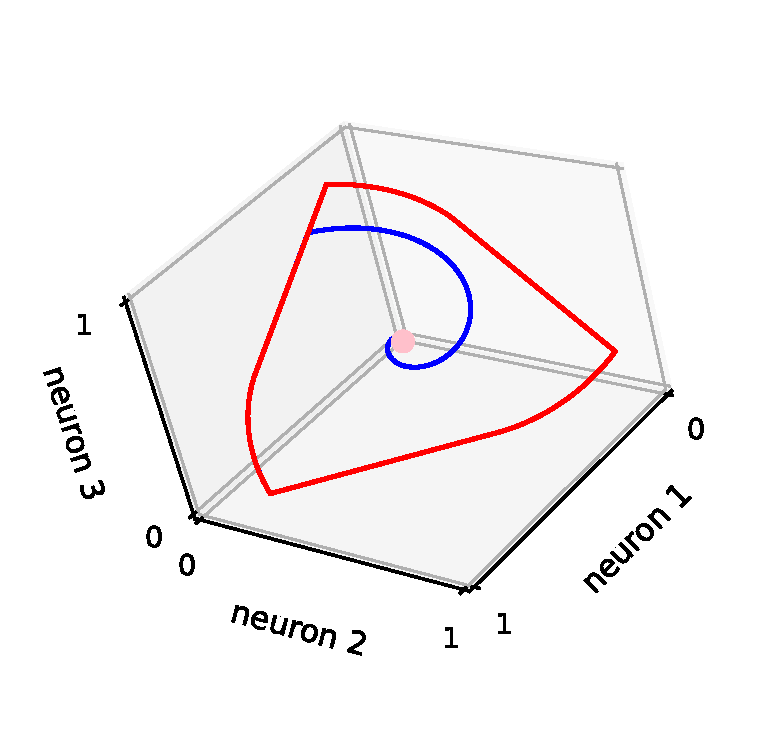
\includegraphics[width=0.8\textwidth]{figures/bpa3_limitcycle_single.pdf}
    \caption{Limit cycle emerging from a perturbation of the bounded plane attractor.}
    \label{fig:bpa3_limitcycle_single}
\end{figure}


\begin{figure}[H]
    \centering
    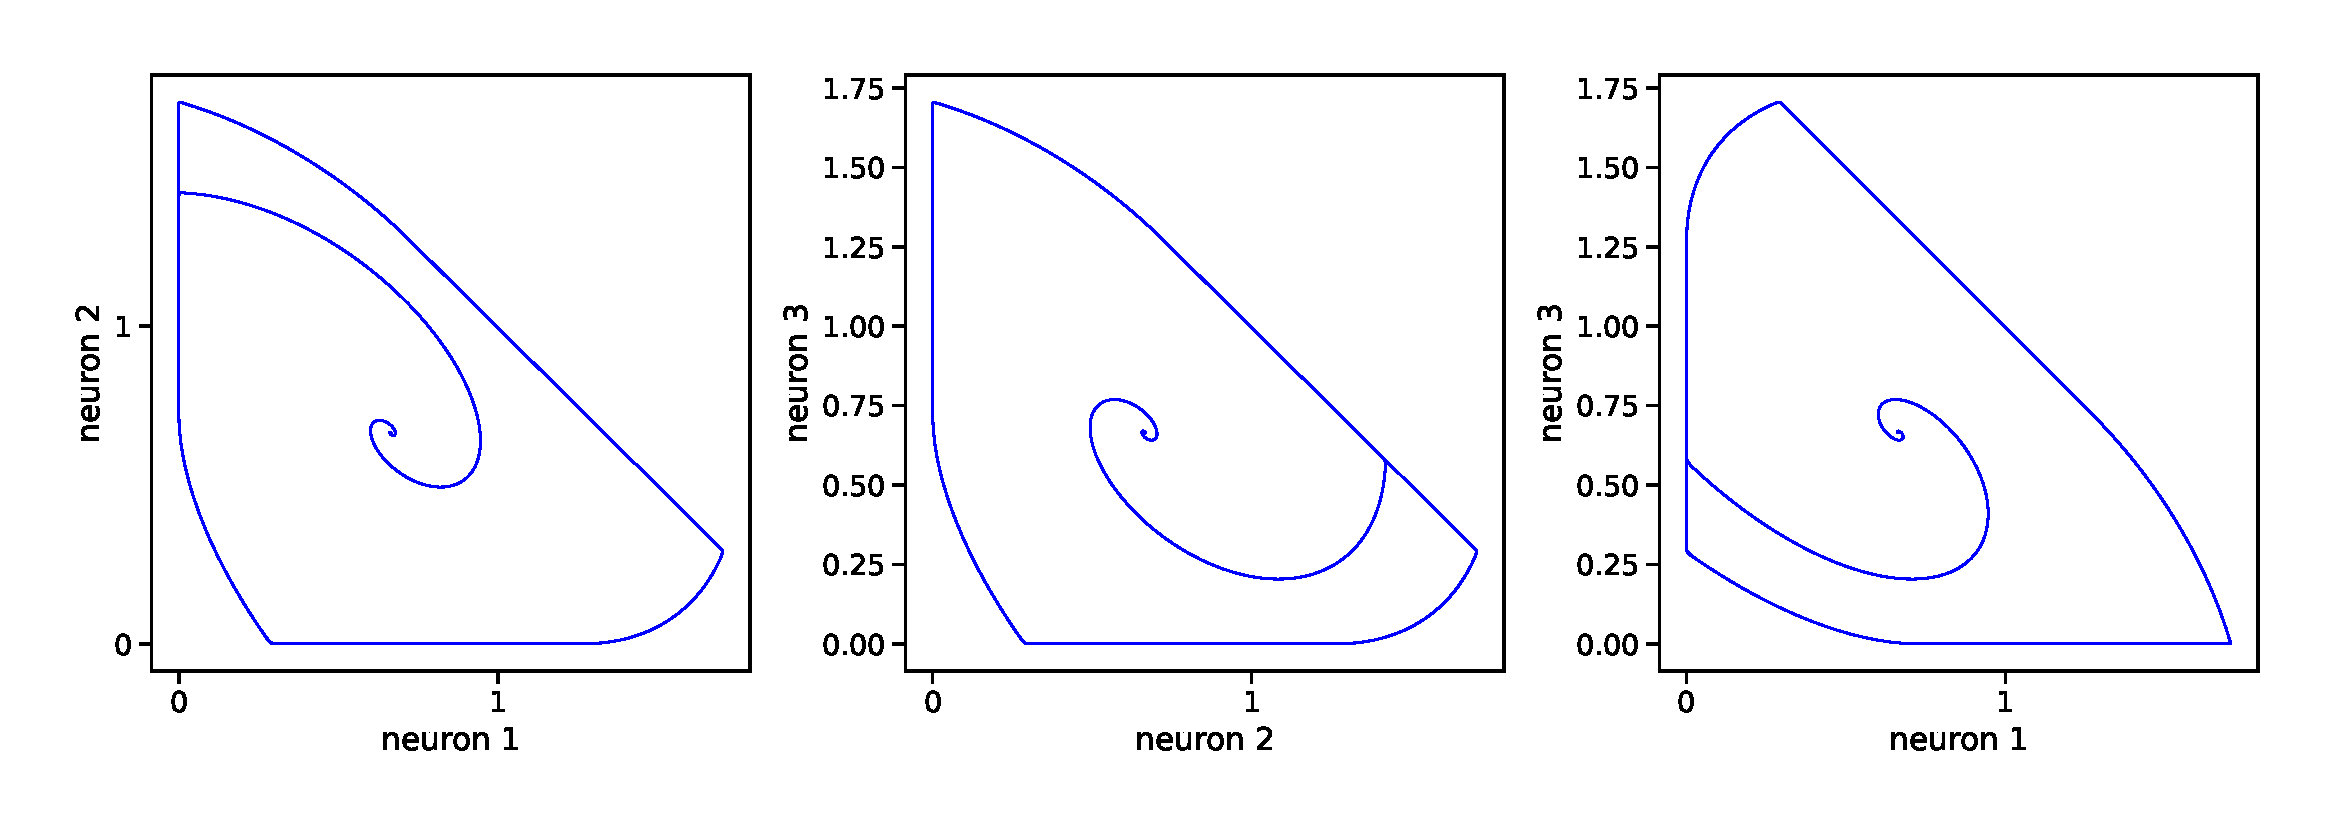
\includegraphics[width=0.99\textwidth]{figures/bpa3_limitcycle_2dproj.pdf}
    \caption{Limit cycle emerging from a perturbation of the bounded plane attractor projected.}
    \label{fig:bla3_limitcycle_single_2d}
\end{figure}


\subsubsection{Existence of limit cycle}
\begin{remark}
Difficult to prove explicitly, for a proof see \citep{bel2021}.
\end{remark}


The set $[0,1]^3$ is a globally attracting set \citep[Lemma 2.1]{morrisonDiversityEmergentDynamics}.

The only fixed point is unstable.
%proof:
Conditions:
Existence %analogues to existence of fixed point with full support 

Uniqueness

Stability


\subsubsection{With four fixed points}
\begin{equation}
\epsilon = 
\begin{pmatrix}
 0  &  -\delta_1 &  0 \\
 0  &  0 & -\delta_1 \\
-\delta_1 & 0 & 0 \\
\end{pmatrix}
\end{equation}
with $\delta_1=\tfrac{1}{100}$.

\begin{figure}[H]
    \centering
    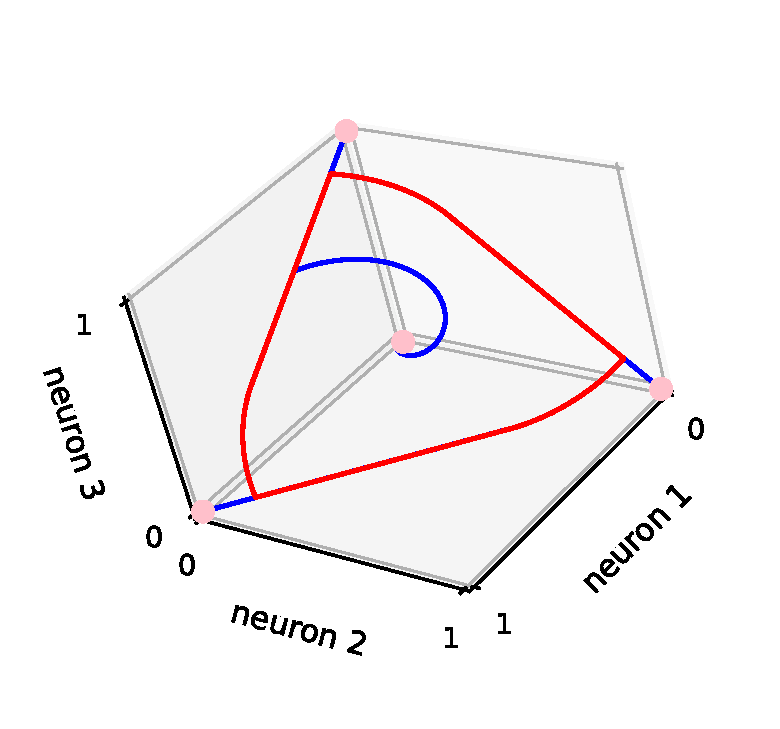
\includegraphics[width=0.8\textwidth]{figures/bpa3_limitcycle_triple.pdf}
    \caption{Limit cycle emerging from a perturbation of the bounded plane attractor.}
    \label{fig:bpa3_limitcycle_triple}
\end{figure}

\begin{figure}[H]
    \centering
    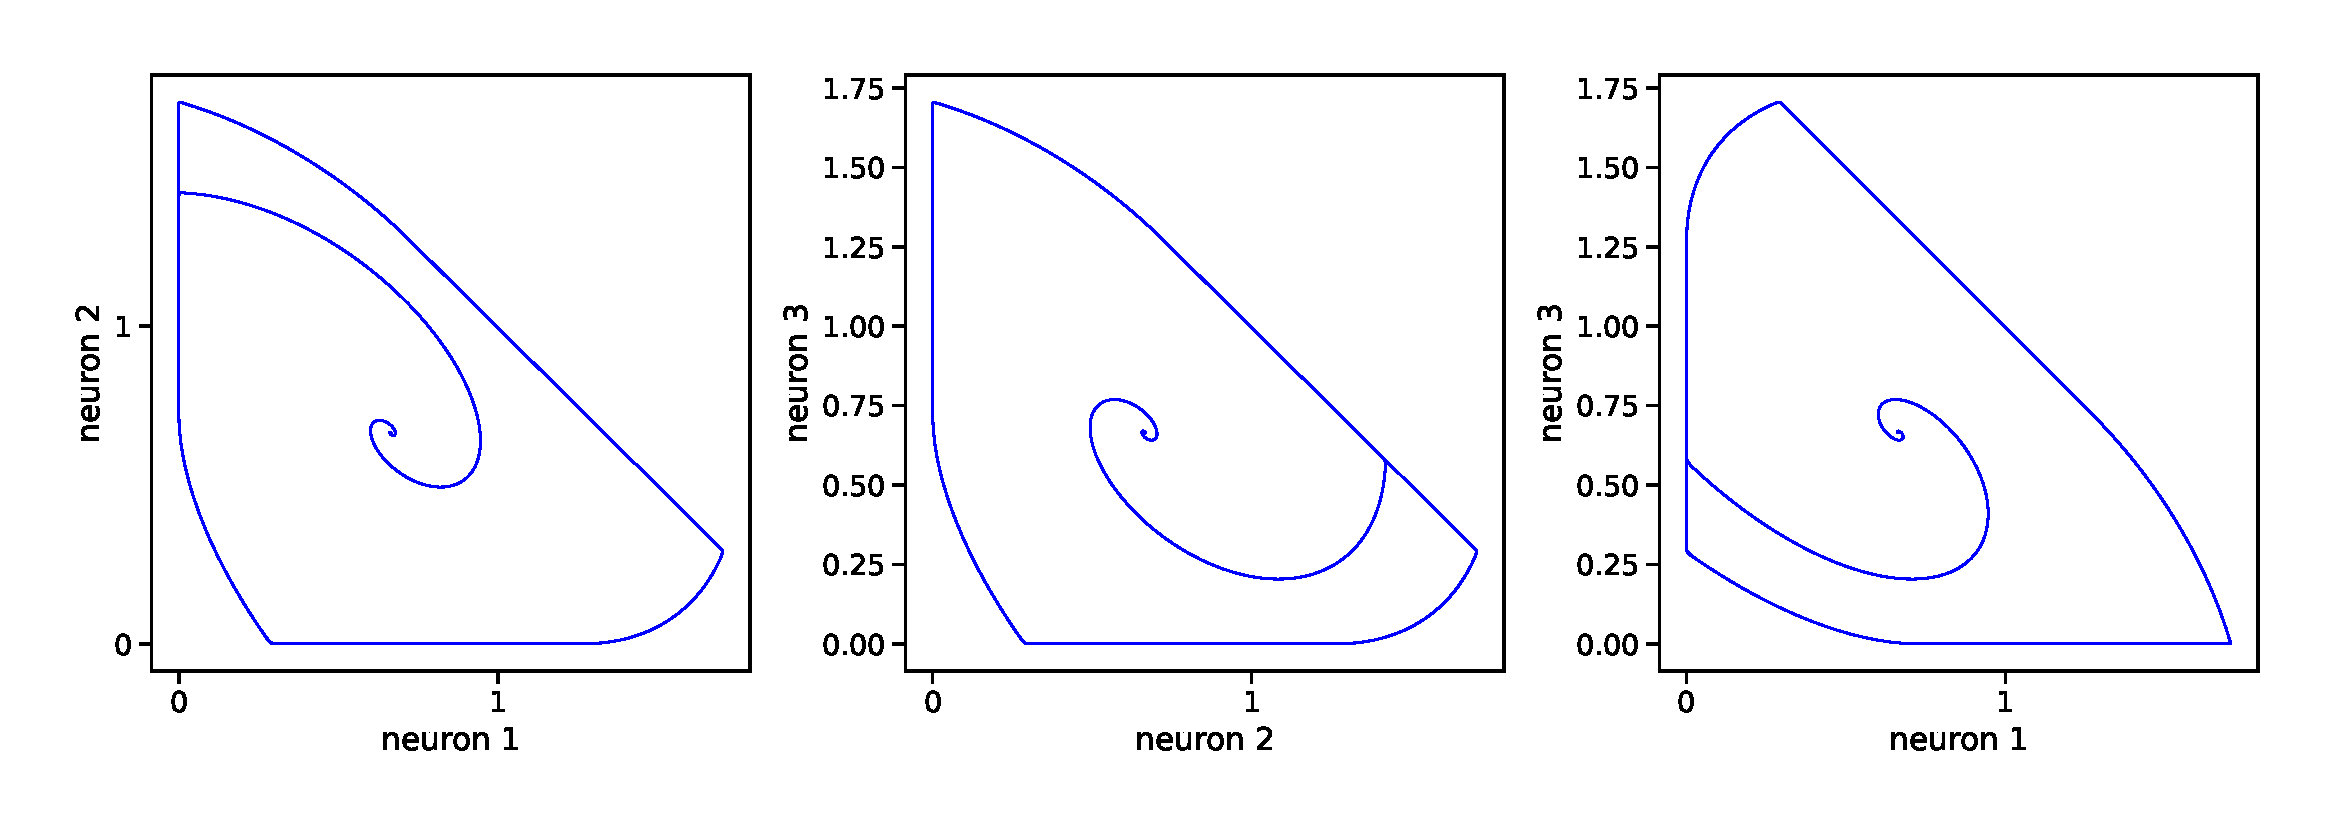
\includegraphics[width=0.99\textwidth]{figures/bpa3_limitcycle_2dproj.pdf}
    \caption{Limit cycle emerging from a perturbation of the bounded plane attractor projected.}
    \label{fig:bla3_limitcycle_triple_2d}
\end{figure}


\subsection{Harmonic oscillator}
\begin{equation}
\epsilon = 
\begin{pmatrix}
 0  &  -\delta_1 & \delta_1 \\
 \delta_1  &  0 & -\delta_1 \\
-\delta_1 & \delta_1 & 0 \\
\end{pmatrix}
\end{equation}

\subsection{Bounded line attractor}
\begin{figure}[H]
    \centering
    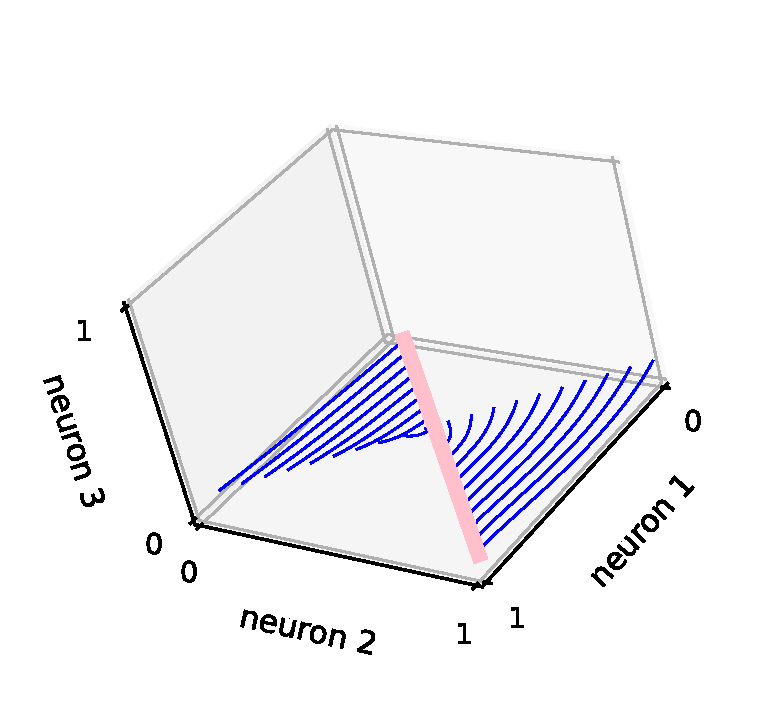
\includegraphics[width=0.8\textwidth]{figures/bpa3_bla.pdf}
    \caption{Bounded line attractor emerging from a perturbation of the bounded plane attractor.}
    \label{fig:bpa3_bla}
\end{figure}


\begin{figure}[H]
    \centering
    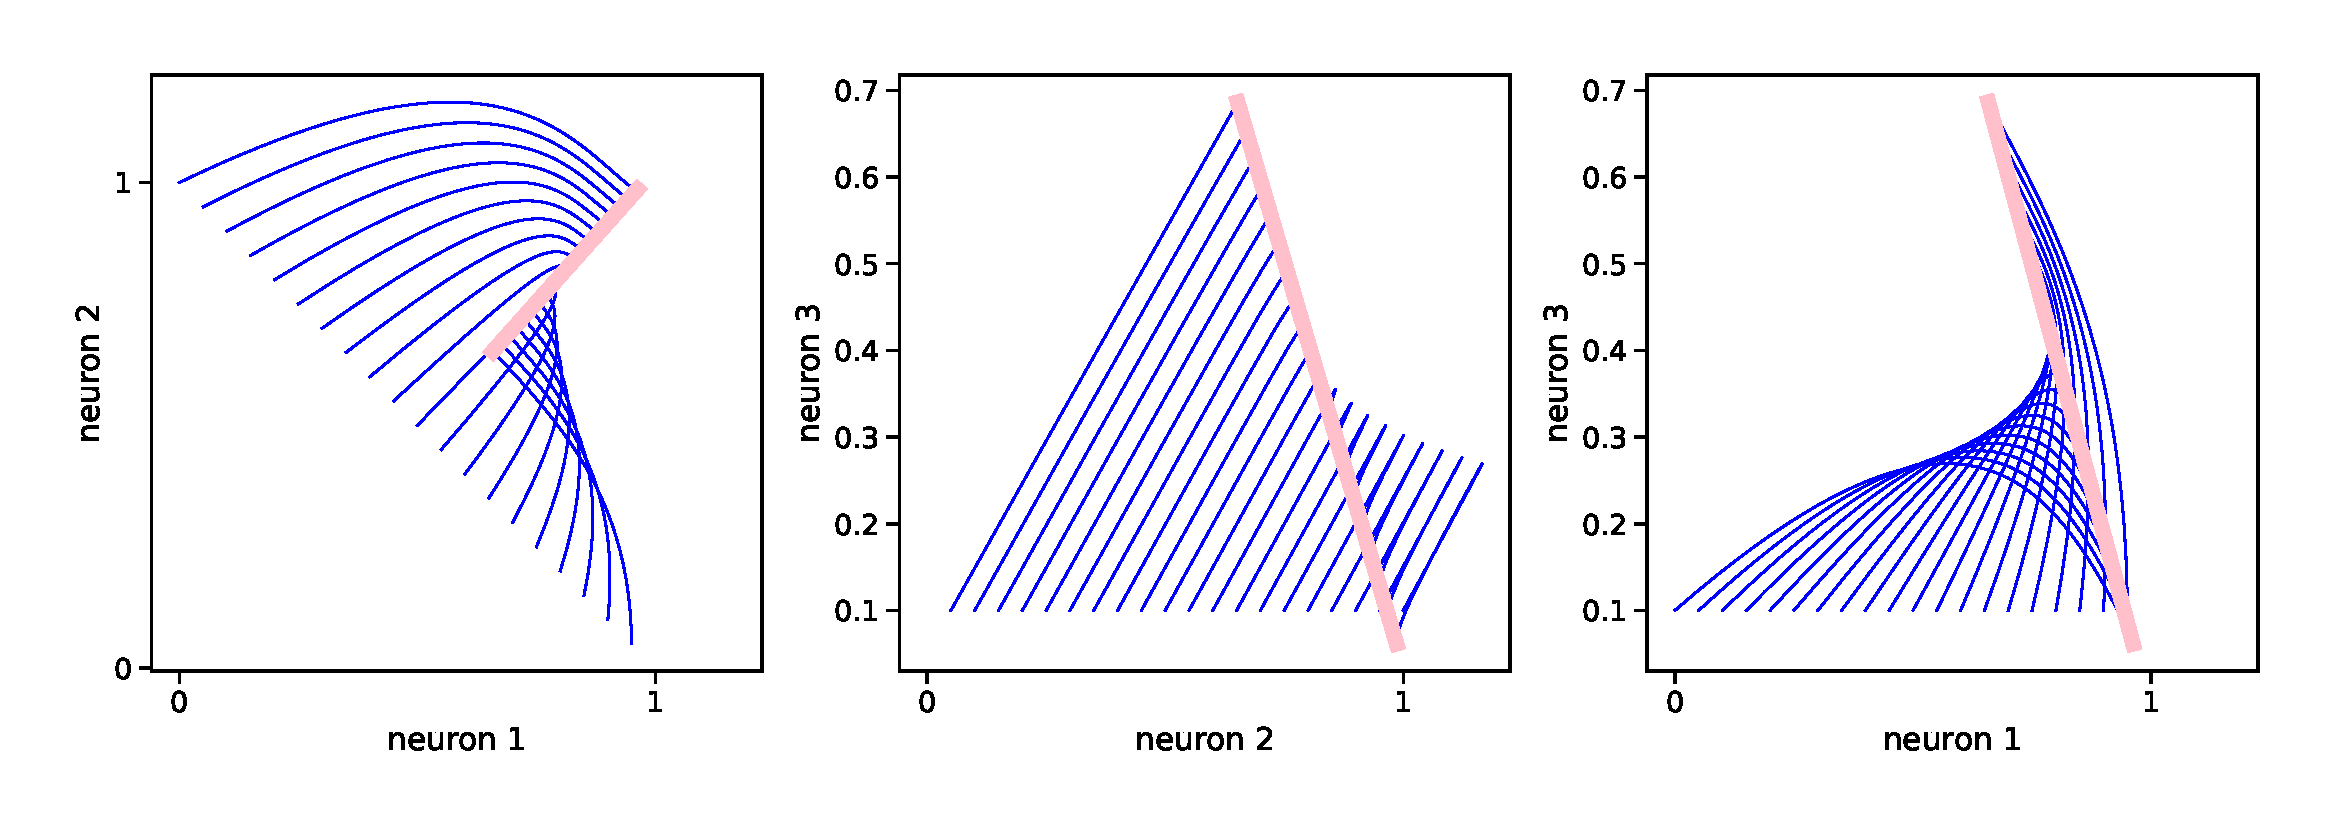
\includegraphics[width=0.99\textwidth]{figures/bpa3_bla_2dproj.pdf}
    \caption{Bounded line attractor emerging from a perturbation of the bounded plane attractor projected.}
    \label{fig:bla3_bla_2d}
\end{figure}


% \newpage
\addcontentsline{toc}{section}{References}
\bibliographystyle{plain}
\bibliography{cit.bib, CITCOD.bib}

%\bibliography{/Users/abel_/Documents/Rotations/CIT/cit_for_computation/Stability/CIT-for-Computation.bib,
%/Users/abel_/Documents/Rotations/CIT/cit_for_computation/Stability/cit.bib, 
%/Users/abel_/Documents/Rotations/CIT/cit_for_computation/Stability/CITCOD.bib}

\end{document}